
\chapter{Impossible languages}

% TODO: rewrite opener -- mild AI-tic cluster
% TODO: confirm wordplay -- is "ingrammatical" intentional alongside "antigrammatical"?
Linguists have ventured into the realm of impossible languages, crafting systems that are ungrammatical -- ingrammatical, antigrammatical -- by their very nature. These languages defy the syntactic structures we're familiar with, presenting sentences where words are arranged in random sequences, obliterating any semblance of conventional order. They experiment with grammatical rules based on the numerical position of words or on fully or partially backward sequences. These linguistic constructs stretch the definition of language, inhabiting a space that's scarcely linguistic at all.

\begin{quote}
    In one language, for instance, any string is grammatical as long as its length is prime: any five-word string is in the language, any six-word string is out. Or consider the language where the rule is that any word that occurs in a sentence must occur an even number of times. So, if we use different letters to represent different words, the sequence abbcabcb is grammatical, while bbbcabcb is ungrammatical. \hfill\citep[54]{Sampson1975}
    % TODO: write transitions between Sampson block quotes -- currently stitched with bare \dots
    \dots
    The trouble is that if we use transformations, we can define any kind of language that can be defined at all. I have been talking about ps grammars, transformations, and so on in quite a woolly, intuitive way, but one can make these notions precise and rigorous. If one defines the notion transformational grammar precisely, there is a theorem that any rel can be defined by some transformational grammar. In other words, even the ridiculous case of the prime number language I discussed earlier, which, we agreed, could never occur as a natural language, could be specified by some transformational grammar.
    % TODO: write transitions between Sampson block quotes -- currently stitched with bare \dots
    \dots
    So, although the theory of transformational grammar does not partition the set of rel's into a set of possible and a set of impossible languages, it does impose an ordering on the languages, so that some of the rel's will be relatively easy to describe with transformational notation and other rel's will be much harder to define that way (even though they might be quite easy to define in some other notation system). There are all kinds of notation systems one could imagine, each of which would permit all the rel's to be defined; but, depending which notation system one chooses, one gets a different complexity ordering among the various rel's. If it is empirically true that, in the ordering defined by Chomsky's particular notation system, all the natural languages are relatively near the simple end of the range, then Chomsky's notation must correspond to % TODO: OCR error -- original Sampson 1975 word unrecoverable from this transcription; verify against source
    EJiiirt contingent fact about the nature of natural language. Now it might be the case that there is some feature of the environment, outside the human organism, which forces this structure on the languages that humans use. But % TODO: complete the Sampson quote or trim to a coherent stopping point
    \hfill\citep[56]{Sampson1975}
\end{quote}

% TODO: verify Moro 2016 attribution -- sentences look like quoted material; mark with \enquote{} or convert to block quote if so
To make a negative clause, place \mention{no} after the third word of the clause. The first article of the clause has to agree with the last noun. A closed interrogative clause is formed by inverting the order of the corresponding declarative clause. \citep[55--56]{Moro2016}

% TODO: develop into bridge paragraph
What could this be for?

Sometimes, the best way to clarify something is to imagine what it's not. The hugely influential linguist Noam \textcite{Chomsky1957} believed that some sentences belong to a particular language and other sequences of words don't. But beyond that, he believed the strings that don't can be further subdivided into those that \emph{could} be part of the particular language, and those that simply \emph{couldn't}. To make that more concrete, various ideas have been floated about what these impossible languages might be like.
% EDITORIAL-HPC: Keep the formal-language history, but do not let this chapter
% define grammaticality by generability or statistical probability. Use it to
% show constraints on possible maintenance/projectibility, not to replace the
% detector/coupling account.

For example, in (\ref{ex:even-odd-shuffle}), all the even-numbered words are fronted, preserving their original order. In (\ref{ex:partial-reverse}), a special character is inserted, after which everything is reversed. And in (\ref{ex:tense-hop}), the tense-marker on any verb attaches to the word four positions to the right of the verb (or less if fewer words are available). Figure \ref{fig:imp-possible-languages} puts these and other perturbations on an impossible--possible continuum of these languages.

\ea
    \ea[]{\textit{He cleans all the books on his very messy bookshelf.}\hfill[English]} \label{ex:unperturbed}
    \ex[]{\textit{He all books his messy cleans the on very bookshelf.}\hfill[Even-Odd]}\label{ex:even-odd-shuffle}
    \ex[]{\textit{He cleans all the books on }|\textit{ bookshelf messy very his.}\hfill[Partial reverse]}\label{ex:partial-reverse}
    \ex[]{\textit{He clean all the books on\myuline{s} his very messy bookshelf.}\hfill[Tense hop]}\label{ex:tense-hop}
    \z
\z

\begin{figure}
    \centering
    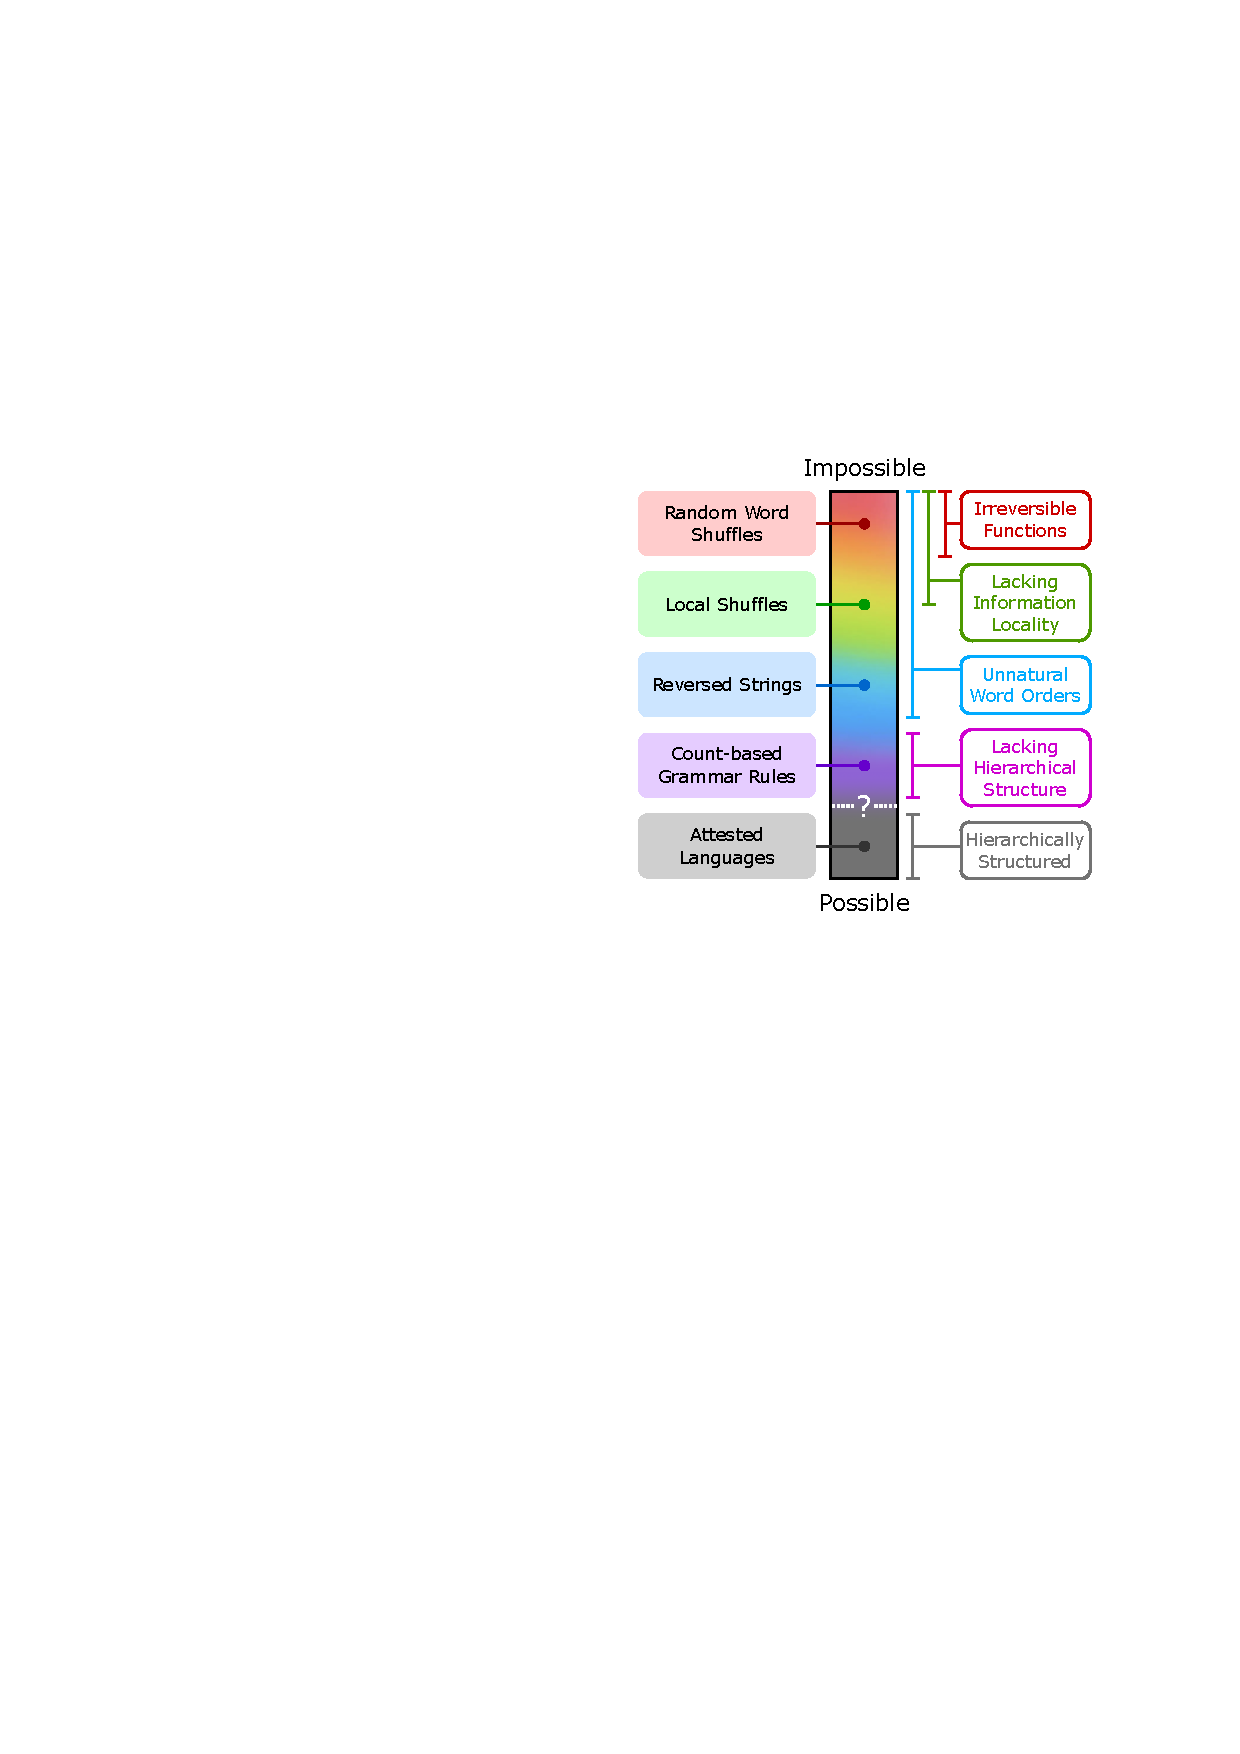
\includegraphics{figures/impossible-languages.pdf}
    % TODO: secure CC-BY downstream-reuse rights for Kallini 2024 Figure 1
    \caption{Partial impossibility continuum of languages based on complexity. Reproduced from \textcite{Kallini2024} Figure 1.}
    \label{fig:imp-possible-languages}
\end{figure}



\ea \label{ex:greenIdeas}
    \ea[]{\textit{Colorless green ideas sleep furiously.}}
    \label{ex:greenIdeas1}
    \ex[*]{\textit{Furiously ideas sleep green colorless.}}
    \label{ex:greenIdeas2}
    \z
\z

\begin{figure}
    \centering
    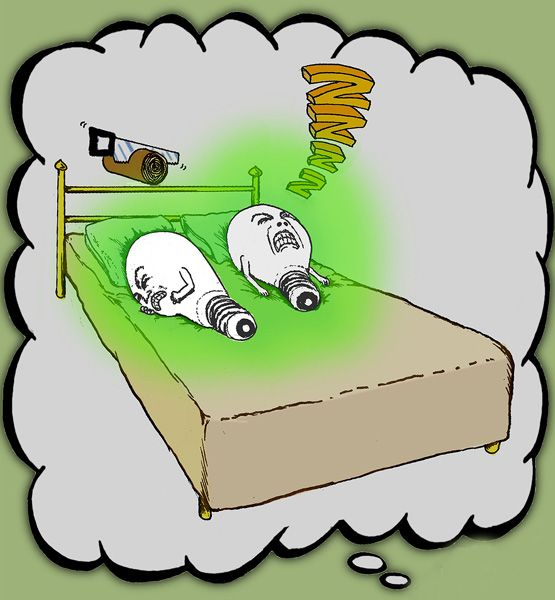
\includegraphics[width=3in]{figures/green-ideas.jpg}
    % TODO: secure permission for Parkvall cartoon reproduction
    \caption{A cartoon showing angry lightbulbs with green glows sleeping, from Mikael Parkvall's \textit{Limits of Language}.}
    \label{fig:greenIdeas}
\end{figure}

\textcite[16]{Chomsky1957} claims that neither (\ref{ex:greenIdeas1}) nor (\ref{ex:greenIdeas2}), nor their subparts, would occur in a corpus of English, they would be \enquote{equally \enquote*{remote} from English [\dots] in any statistical model of English} and that they're equally ungrammatical. But Fernando \textcite{Pereira2000} showed that (\ref{ex:greenIdeas1}) is much more statistically likely than (\ref{ex:greenIdeas2}), which matches my intuition (and yours too, perhaps).

% TODO: write closing beat -- chapter currently ends without a hand-off to the next
